\chapter{TacOSのファイルシステム}
\label{tacosFAT}

TacOSのファイルシステムサーバ(fs)\footnote{
  \url{https://github.com/tctsigemura/TacOS/tree/master/os/fs}
}のプログラムを用いて,
FATファイルシステムの実装例を示す.
ファイルシステムサーバのクラス図を\figref{fsUML}に示す.
ファイルシステムサーバは,
サーバプロセスのメインルーチン(fsクラス\footnote{
  \url{https://github.com/tctsigemura/TacOS/blob/master/os/fs/fs.cmm}
  (\texttt{fs.hmm})}),
システムコールを処理する(fatSysクラス\footnote{
  \url{https://github.com/tctsigemura/TacOS/blob/master/os/fs/fatSys.cmm}
  (\texttt{fatSys.hmm})}),
オープン済みファイル毎にバッファを割付け,
バイト単位の操作を提供する上位のファイルシステム(fileクラス\footnote{
  \url{https://github.com/tctsigemura/TacOS/blob/master/os/fs/file.cmm}
  (\texttt{file.hmm})}),
ディレクトリの管理を行う(dirAccessクラス\footnote{
  \url{https://github.com/tctsigemura/TacOS/blob/master/os/fs/dirAccess.cmm}
  (\texttt{dirAccess.hmm})}),
FATを管理し,
セクタ単位の操作を提供する下位のファイルシステム(blkFileクラス\footnote{
  \url{https://github.com/tctsigemura/TacOS/blob/master/os/fs/blkFile.cmm}
  (\texttt{blkFile.hmm})}),
デバイスドライバ(mmcspiクラス\footnote{
  \url{https://github.com/tctsigemura/TacOS/blob/master/os/fs/mmcspi.cmm}
  (\texttt{mmcspi.hmm})})
からなる.

\begin{myfig}{btp}{TacOSのファイルサーバの構造}{fsUML}
  \centering{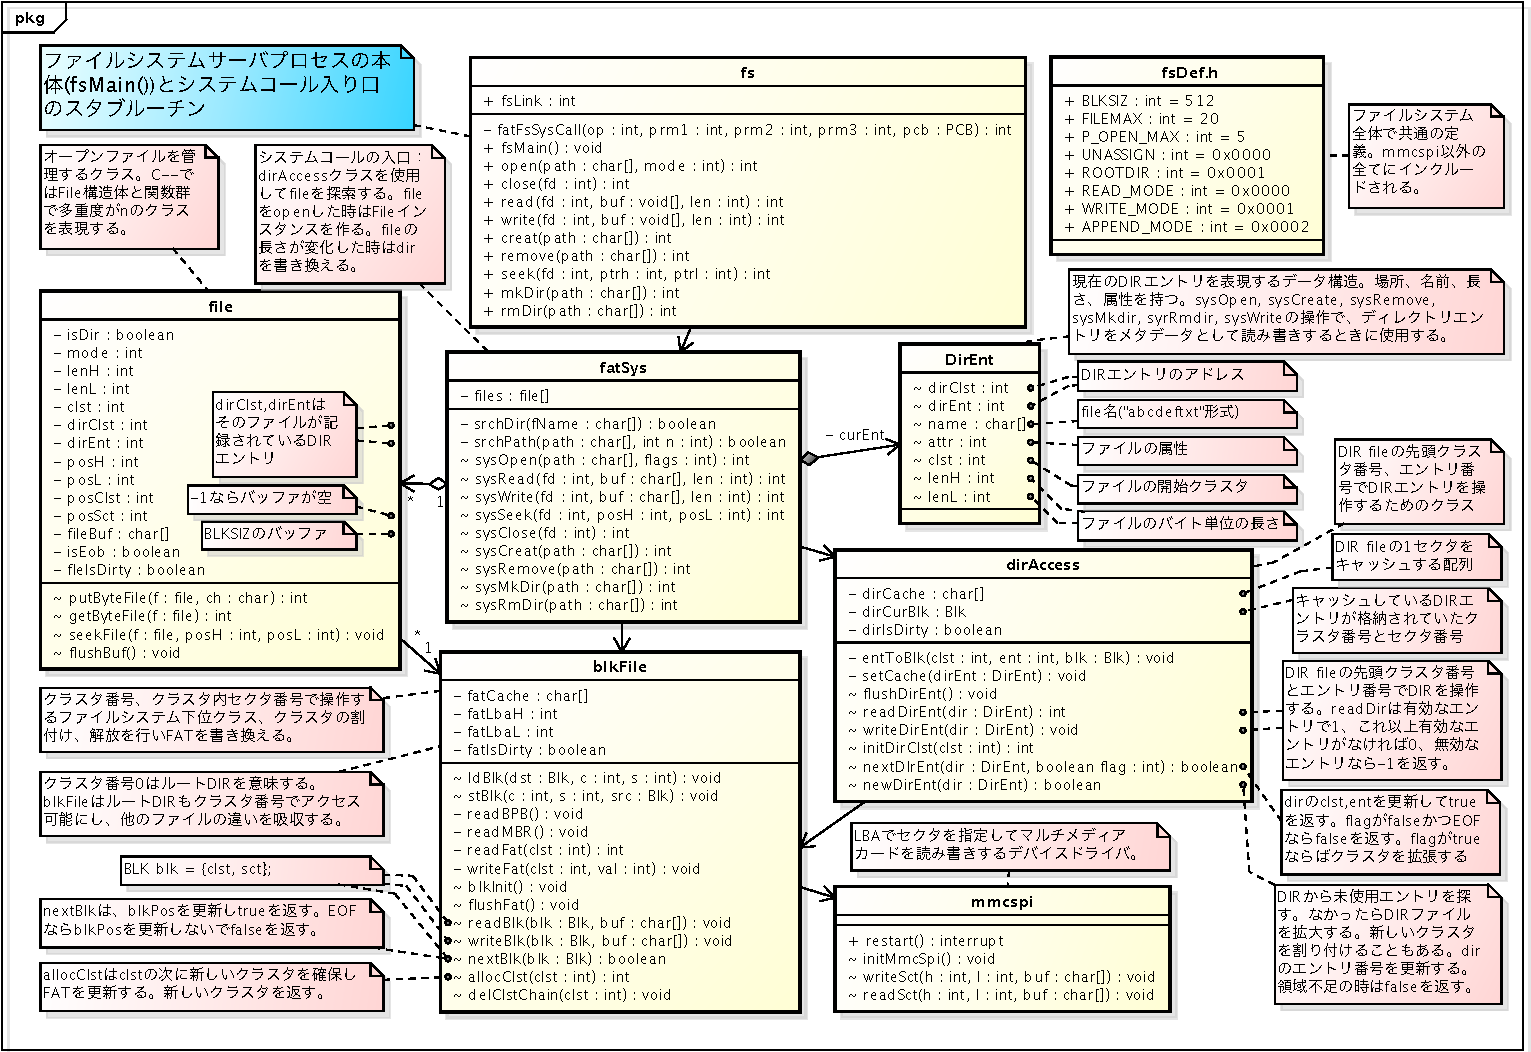
\includegraphics[scale=0.84,angle=90]{TacOS/uml/fs-crop.pdf}}
\end{myfig}

%============================================================================
\section{fsクラス}
fsクラスはファイルサーバプロセスのメインループと,
他のプロセスが呼び出すシステムコールのスタブルーチンを持っている.

\begin{itemize}
\item \emph{サーバプロセス}\\
  リスト\ref{tacosFsMain}に示す\|fsMain()|が
  サーバプロセスのメインルーチンである.
  リンクを作成した後,無限ループでメッセージの受信と返信を繰り返す.
  \|receive()|,\|send()|は第\ref{tacosIPC}章で紹介した
  TacOSのメッセージ通信機構である.
  \|fatFsSysCall()|は,
  システムコールの種類に応じてfatSysクラスの関数を呼び出す.
  \|fatFsSysCall()|の一部をリスト\ref{tacosFatFsSysCall}に示す.
  \lstinputlisting[caption=ファイルシステムサーバのメインループ(fsMain()),
    firstline=87,lastline=97,numbers=none,
    label=tacosFsMain,float=btp]{TacOS/fs/fs.cmm}
  \lstinputlisting[caption=システムコールによって分岐する(fatFsSysCall()),
    firstline=63,lastline=68,numbers=none,
    label=tacosFatFsSysCall,float=btp]{TacOS/fs/fs.cmm}
\item \emph{スタブルーチン}\\
  \|open()|〜\|rmDir()|は,
  システムコールを発行する側のプロセスが呼び出す.
  これらの関数はシステムコールを実際に処理をするのではなく,
  ファイルシステムサーバにメッセージを送信するだけのスタブである.
  スタブの例として\|open()|関数をリスト\ref{tacosOpen}に示す.
  \|sendrec()|はサーバプロセスの\|receive()|,\|send()|と通信する
  TacOSのメッセージ通信機構の関数である.
  \lstinputlisting[
    caption=クライアントプロセスが呼び出すスタブルーチンの例(open()),
    firstline=128,lastline=132,numbers=none,
    label=tacosOpen,float=btp]{TacOS/fs/fs.cmm}
\end{itemize}

%============================================================================
\section{fatSysクラス}
ファイルシステムのシステムコールを処理するクラスである.
fileクラス,dirAccessクラス,blkFileクラスの機能と,
fatSysクラス自身が持つパスの解析機能とオープン中ファイルの管理機能を使用して,
システムコールを実行する.

\begin{itemize}
\item \emph{ディレクトリファイル内の探索} \\
  ディレクトリファイルを指定し,ファイル名でエントリを探索する関数は,
  リスト\ref{tacosSrchDir}の\|srchDir()|関数である.
  \|srchDir()|関数は,
  現在の着目位置から始めて指定された名前のエントリを探索する.
  着目位置は,\|DirEnt|型(\figref{fsUML}およびリスト\ref{tacosDirEnt}参照)
  のオブジェクト\|curEnt|に,
  ディレクトリファイルのクラスタ番号とディレクトリエントリの番号として
  記録している.

  \lstinputlisting[caption=ディレクトリファイル内を探索する(srchDir()),
    firstline=158,lastline=171,float=btp]{TacOS/fs/fatSys.cmm}

  dirAccessクラスの\|readDirEnt()|関数は,
  着目位置のディレクトリエントリを\|curEnt|に読み込む.
  \|nextDir()|関数は\|curEnt|の着目位置を一つ進める.

\item \emph{パスの解析} \\
  TacOSにはカレントディレクトリの概念が無いので,
  パスの探索はいつもルートディレクトリから開始する.
  パスの探索はリスト\ref{tacosSrchPath}の\|srchPath()|関数が行う.
  引数は解析するパス(\|path|)と解析する文字数(\|n|)である.
  ファイルが登録されているディレクトリを操作する場合などは,
  パスの途中までを利用することがあるので文字数が必要である.
  
  \lstinputlisting[caption=パスを解析する(srchPath()),
    label=tacosSrchPath,
    float=btp,numbers=left,xleftmargin=5mm, 
    firstline=176,lastline=201]{TacOS/fs/fatSys.cmm}

  ルートディレクトリはクラスタ番号が\|ROOTDIR|(実際の値は\|1|)の
  ファイルとしてblkFileクラスが扱うので,
  \|curEnt|は3行から9行のように初期化する.
  13行でパスの先頭にある余分な\|/|を取り除き),
  解析位置がパスの最後まで来ていたら終了である(14行).
  着目しているディレクトリファイルのクラスタ番号を,
  新しく見つけたファイル(次の階層のディレクトリファイル)の
  開始クラスタ番号で置換える(18行).
  これにより,着目しているディレクトリが次の階層のものになる.
  探索中のパス名から次の階層のファイル名を取出し(22行),
  着目しているディレクトリファイルの中を,
  前出の\|srchDir()|関数を用いて探索する(23行).
  もしも,名前が見つからなければ終了するし,
  そうでなければ13行に戻る.

\item \emph{オープン中ファイルの管理} \\
  オープンファイル毎にFileクラス(\figref{fsUML}ではfileクラス)の
  オブジェクトを割付けfile配列に登録する.
  ファイルがクロースされるまで,
  ファイル操作はFileオブジェクトを用いて行われる.
  openシステムコールがFileオブジェクトの登録を行うので,
  openシステムコールの処理プログラム\|sysOpen()|を
  リスト\ref{tacosSysOpen}に示す.
  この関数は,
  リスト\ref{tacosFatFsSysCall}の\|fatFsSysCall()|関数から呼び出される.

  2行はクライアントプロセスのPCB中に
  ファイルを記録を残す場所を確保している\footnote{
    プロセス終了時にファイルを自動的にクローズるために,
    プロセス(PCB)に記録を残す必要がある.}.
  4行はfatSysクラスの\|files|配列に場所を確保している.
  7行で前出の\|srchPath()|関数を用いて\|path|を最後まで解析し,
  目的ファイルのディレクトリエントリを探す.
  見つからない場合はエラーになる\footnote{
    TacOSのopenシステムコールにはファイルの作成機能は無い.
    ファイルの作成はcreatシステムコールで行う.}.
  12行でディレクトリファイルも読み出しオープンを可能にしている.
  14〜18行ではFileオブジェクトとセクタを格納するバッファを生成している.

  \lstinputlisting[caption=openシステムコールの本体(sysOpen()),
    label=tacosSysOpen,float=btp,numbers=left,xleftmargin=5mm,
    firstline=234,lastline=273]{TacOS/fs/fatSys.cmm}

  20〜29行ではFileオブジェクトを初期化している.
  21行ではオープンファイルが
  ディレクトリファイルであることを表すブラグをセットしている.
  26〜27行ではオープンファイルが格納されている
  ディレクトリエントリを記録している\footnote{
    FATファイルシステムでは
    ファイルサイズなどをディレクトリエントリに記録しているので,
    ファイルをオープン後もディレクトリエントリにアクセスする必要がある.}.
  
  33行,35行では,Fileオブジェクトを引数にfileクラスの関数を使用してる.
  {\cmml}で,
  fileクラスのような複数のインスタンスを持つクラスを操作する場合,
  インスタンスを引数にクラスの関数を呼び出す.

\item \emph{オープン中ファイルの操作} \\
  オープン中のファイルはFileオブジェクトを用いて操作する.
  例としてreadシステムコールの処理プログラム\|sysRead()|を
  リスト\ref{tacosSysRead}に示す.
  この関数は,
  リスト\ref{tacosFatFsSysCall}の\|fatFsSysCall()|関数から呼び出される.

  \lstinputlisting[caption=readシステムコールの本体(sysRead()),
    label=tacosSysRead,
    float=btp,numbers=left,xleftmargin=5mm,
    firstline=302,lastline=318]{TacOS/fs/fatSys.cmm}

  2行の\|chkIdx()|はプロセスのファイルディスクリプタ番号から,
  Fileクラスのオブジェクトを求める.
  6行は作成後まだクラスタが割り当てられていないファイルの場合の処理である.
  11〜15行ではFileクラスの\|getByteFile()|を用いて,
  ファイルオブジェクトを通してファイルのデータを\|buf[]|に読み出している.

\item \emph{ディレクトリの書き換え} \\
  ディレクトリ書き換え操作の例として,
  ファイルを削除するremoveシステムコールの処理プログラムを
  リスト\ref{tacosSysRemove}に示す.
  この関数は,
  リスト\ref{tacosFatFsSysCall}の\|fatFsSysCall()|関数から呼び出される.

  12行で\|srchPath()|を用いて削除するファイルのディレクトリエントリを探索する.
  14行の\|isOpened()|は,システム中の全オープンファイルについて調べ,
  削除するファイルがオープン中でないか調べる.
  オープン中のファイルは削除できない.
  削除しても構わないなら,16行で\|delFile()|を用いてファイルを消す.
  \|delFile()|はディレクトリの削除(rmdirシステムコール)からも使用される.
  3,7行で使用される\|delClstChain()|,\|flushFat()|はblkFileクラスの関数,
  5,6行の\|writeDirEnt()|,\|flushDirEnt()|はdirAccessクラスの関数である.

  \lstinputlisting[caption=removeシステムコールの本体(sysRemove()),
    label=tacosSysRemove,
    float=btp,numbers=left,xleftmargin=5mm,
    firstline=430,lastline=447]{TacOS/fs/fatSys.cmm}

\end{itemize}

%============================================================================
\section{Fileクラス(fileクラス)}
オープン中のファイルを管理・操作するためのクラスである.
\|file.hmm|にインタフェース,\|file.cmm|に実装が書いてある.
このクラスはオープンファイルの数だけインスタンスが生成される.
オブジェクト指向言語ではない{\cmm}では,
\|file.hmm|中に宣言されている\|File|構造体でインスタンスの属性を表現し,
\|file.cmm|中の関数に引数として属性を渡して処理させることで,
インスタンスの操作を実現している.
インスタンスが複数ある場合は,複数の\|File|構造体インスタンスが生成される.
なお,インスタンスを一つしか持たないクラスの場合は,
属性をスタティク変数として表現すれば十分である.

\begin{itemize}
\item \emph{Fileクラスの仕様}\\
  リスト\ref{tacosFile}にFileクラスの仕様にあたる\|file.hmm|を示す.
  1〜19行の構造体が属性を,21〜24行のプロトタイプ宣言が操作を表現する.
  3〜9行はファイルシステムに書き込まれるファイルの静的な属性である.
  12〜18行はファイルがクローズされると必要なくなる一時的な属性である.
  21〜24行の関数はファイルオブジェクトを引数に実行される.

  \lstinputlisting[caption=Fileクラスの外部インタフェース(file.hmm),
    label=tacosFile,
    float=btp,numbers=left,xleftmargin=5mm,
    firstline=34,lastline=57]{TacOS/fs/file.hmm}

\item \emph{ファイルの読み書き}\\
  例として,ファイルからデータを読み出す\|getByteFile()|を
  リスト\ref{tacosGetByteFile}に示す.
  6行の\|fillBuf()|はファイルオブジェクトのバッファに
  次に読むデータが格納済みか調べ格納されていなかったら,
  blkFileクラスの機能を利用して目的のバイトを含む一セクタを読む.
  
  \lstinputlisting[
    caption=ファイルからバイト単位でデータを読む(getByteFile()),
    label=tacosGetByteFile,float=btp,numbers=left,xleftmargin=5mm,
    firstline=105,lastline=115]{TacOS/fs/file.cmm}

\end{itemize}

%============================================================================
\section{dirAccessクラス}
dirAccessクラスはblkFileクラスの機能を利用して,
ディレクトリエントリを読み書きする機能を提供する.
fatSysクラスはパスの解析や,
ファイルの作成・削除,ファイルサイズの変更等でディレクトリの操作で,
dirAccessクラスの機能を利用する.

\begin{itemize}
\item \emph{ディレクトリエントリのキャッシュ} \\
  dirAccessクラスはディレクトリエントリを含むセクタを\|dirCache|に
  キャッシュし,メディアに対するアクセス回数を減らす工夫をしている.
  \|dirCurBlk|,\|dirIsDirty|(クラス図参照)は,
  キャッシュを管理するためのデータである.

\item \emph{ディレクトリエントリ構造体} \\
  リスト\ref{tacosDirEnt}に示す
  \|DirEnt|構造体はディレクトリエントリの読み書きに使用される.
  \|dirClst|,\|dirEnt|がディレクトリファイルとファイル内の位置であり,
  ディレクトリエントリのアドレスを表現している.
  4行以下はディレクトリエントリの内容である.

  \lstinputlisting[caption=ディレクトリエントリ構造体(DirEnt),
    label=tacosDirEnt,float=btp,numbers=left,xleftmargin=5mm,
    firstline=34,lastline=42]{TacOS/fs/dirAccess.hmm}

\item \emph{ディレクトリエントリの読み書き} \\
  例として,ディレクトリファイル(またはルートディレクトリ)から
  エントリを読み出す\|readDirEnt()|をリスト\ref{tacosReadDirEnt}に示す.

  \lstinputlisting[
    caption=ディレクトリファイルからエントリを読む(readDirEnt()),
    label=tacosReadDirEnt,float=btp,numbers=left,xleftmargin=5mm,
    firstline=96,lastline=111]{TacOS/fs/dirAccess.cmm}

  \|readDirEnt()|関数は,
  \|DirEnt|型の引数\|dirEnt|にディレクトリファイルの位置と
  ディレクトリファイル内のエントリ番号を格納して呼出される.
  5行で,目的のディレクトリエントリがキャッシュに存在しない時,
  ディレクトリエントリを含むセクタを\|dirCache|配列に読込む.
  6行は,目的のエントリの\|dirCache|配列中の位置を\|curEnt|に計算する.

  7行は,ファイル名の第1バイトを\|c|に読込む.
  \|c|の値によりエントリの状態を確認し(8,9行),
  有効なエントリの場合は内容を引数の\|dirEnt|構造体に読み込む(10行以降).
  ファイル名の読み出しにはリスト\ref{tacosReadFname}の
  \|readFname()|関数を用いる.
  11行で使用している\|ord()|は
  文字型を整数型に変換する{\cmml}の演算子である.

  12行から14行で使用している\|wordLE()|は
  文字(バイト)配列からリトルエンディアンの
  16ビットデータを読取るマクロである.
  {\cmml}には32ビット整数型がないので,
  ファイル長は2つの16ビット整数(\|lenH|, \|lenL|)で表現する.
  FATファイルシステムは\emph{リトルエンディアン}である.
  下位桁の方がバイト位置では前になっている(13,14行).
\end{itemize}

%============================================================================
\section{blkFileクラス}
\label{readBlkFile}
mmcspiクラスの機能を利用して,
クラスタチェインを辿りながら\emph{セクタ単位}でファイルを読み書きする機能と,
FATにクラスタを割り当てたりクラスタチェインを削除する機能を,
dirAccessクラス,fileクラス,fatSysクラスに提供する.
また,特別なクラスタ番号(\|ROOTDIR=0x0001|)を用いて
ルートディレクトリをファイルのように読み書きする機能も提供する.

\begin{itemize}
\item \emph{初期化}\\
  FATの位置,ルートディレクトリの位置,データ領域の位置等の
  基本情報(リスト\ref{tacosBPB})を,
  \|readMBR()|(リスト\ref{tacosReadMBR})と
  \|readBPB()|(リスト\ref{tacosReadBPB})を使用して求める.
  これらの位置は32ビットのLBAなので,int型の配列で表現する.

  \lstinputlisting[caption=BPB基本情報(blkFile.cmm),
    firstline=75,lastline=80,numbers=left,xleftmargin=5mm,
    label=tacosBPB,float=btp]{TacOS/fs/blkFile.cmm}

  \begin{itemize}
  \item \|readMBR()|はマイクロSDカードのLBA0(MBR)を読み,
    パーティションテーブルを解析してTacOSが扱えるFAT16パーティションを探す.
    パーティションテーブルエントリの構造は,
    \figref{partitionTable}や\tabref{partitionTableEntry}に示した.
    見つけたパーティションの位置をリスト\ref{tacosBPB}の\|bpbLba|に格納する.
  
    \lstinputlisting[caption=MBRを読む(readMBR()),
      firstline=84,lastline=99,numbers=left,xleftmargin=5mm,
      label=tacosReadMBR,float=btp]{TacOS/fs/blkFile.cmm}

    \begin{description}
    \item[2行] \|buf|にセクタを読み出すための512バイトのバッファを確保する.
    \item[3行] mmcspiクラスの\|readSct()|関数を用いて\|buf|にMBRを読み込む.
    \item[5行] MBRの第446バイトからパーティションテーブルが始まる.
      パーティションテーブルエントリのサイズは16バイトである.
    \item[6行] エントリの先頭の\|Flag|を読む.
    \item[7行] エントリの4バイト目の\|Type|を読む.
    \item[9行] TacOSはFAT16パーティションにインストールされているので探す.
    \item[10行] FAT16パーティションが見つかったら,
      エントリの8バイト目から格納されている32ビットの\|Start LBA|を読み出す.
      エントリにLBAはリトルエンディアンで格納されているので,
      上位ワードを10バイト目,下位ワードを8バイト目から読み出している.
      読み出したLBAは\|bpbLba|に格納する.
    \item[11,12行] FAT16パーティションを見つけたので
      バッファを解放して終了する.
    \end{description}

  \item \|readBPB()|は\|bpbLba|を参照しFATのBPB領域の位置を知り,
    BPBの内容を解析する.
    BPBの構造は,\tabref{fatBpbParam}に示した.
    解析結果は,リスト\ref{tacosBPB}の\|fatLba|,
    \|rootLba|,\|dataLba|に格納する.
  
  \lstinputlisting[caption=BPBを読む(readBPB()),
    firstline=102,lastline=128,numbers=left,xleftmargin=5mm,
    label=tacosReadBPB,float=btp]{TacOS/fs/blkFile.cmm}

    \begin{description}
    \item[2行] \|buf|にセクタを読み出すための512バイトのバッファを確保する.
    \item[4行] mmcspiクラスの\|readSct()|関数を用いて\|buf|にBPBを読み込む.
    \item[5行] BPBの11バイト目からの2バイトを読みセクタ長を調べる.
    \item[8行] 13バイト目からクラスタあたりのセクタ数が分かる.
    \item[11,12行] 14バイト目からの2バイト(予約セクタ)は,
      パーティション先頭からFAT開始位置の間のセクタ数である.
      最低でもBPBを格納するために1セクタが予約されている.
      \|bpbLba|に加えFATの位置を計算する.
    \item[15行] FATの大きさをセクタ単位で求める.
    \item[19,20行] FAT数を読み出しFATのセクタ数(\|sctPrFAT|)を掛ける.
      その結果を\|fatLba|に加えることで,
      ルートディレクトリの位置\|rootLba|を計算する.
    \item[23,24行] 17バイト目からの2バイトから
      ルートディレクトリのエントリ数が分かる.
      エントリは32バイトなのでセクタ(512バイト)に16エントリ格納できる.
      16で割ってセクタ数に換算し\|rootLba|に加えることで
      データ領域の開始位置\|dataLba|を求める.
    \item[26行] バッファを解放して終了する.
    \end{description}

  \end{itemize}

\item \emph{クラスタの読み書き}\\
  例としてクラスタを読む\|readBlk()|をリスト\ref{tacosReadBlk}に示す.
  クラスタ番号とクラスタ内セクタ番号(\|Blk|構造体で表現)を
  アドレスとして用い,
  セクタ単位でファイル本体を読む機能を提供する.
  クラスタ番号が\|ROOTDIR|(値は\|0x0001|)の場合は,
  クラスタではなくルートディレクトリ領域のセクタを読む(7〜10行).

  普通のクラスタを読む場合は
  クラスタ番号からセクタ番号へ変換する計算を行う(12〜16行).
  クラスタ番号から2を引いている(12行)のは,
  普通のクラスタ番号は2から始まる(\tabref{fatClsNum}参照)からである.

  セクタ番号が決まったら,
  mmcspiクラス(デバイスドライバクラス)の\|readSct()|を用いて
  セクタを\|buf|に読み込む.

  \lstinputlisting[
    caption=ファイルのデータセクタを読む(readBlk()),
    firstline=195,lastline=213,numbers=left,xleftmargin=5mm,
    label=tacosReadBlk,float=btp]{TacOS/fs/blkFile.cmm}

\item \emph{クラスタチェインの操作}\\
  FAT上のクラスタチェインを操作する三つの機能を準備している.
  \|allocClst()|は,新しいクラスタをクラスタチェインの最後に追加する.
  \|delClstChain()|は先頭クラスタを指定してチェイン全体を削除する.
  \|nextBlk()|は \|Blk|構造体のアドレス(セクタアドレス)を一つ進める.

  クラスタチェインを操作する例として,
  \|Blk|構造体のアドレスを一つ進める役割を持つ
  \|nextBlk()|をリスト\ref{tacosNextBlk}に示す.
  6行でセクタ番号を一つ進める.
  もしもセクタ番号がクラスタの最後まで進んでいれば,
  FATを参照して次のクラスタ番号を求める.
  10行の\|readFat()|がFATを読む関数である.

  \lstinputlisting[
    caption=データセクタのアドレスを進める(nextBlk()),
    firstline=235,lastline=251,numbers=left,xleftmargin=5mm,
    label=tacosNextBlk,float=btp]{TacOS/fs/blkFile.cmm}

\item \emph{FATのキャッシュ}\\
  多くのFATファイルシステムの実装ではFAT全体を主記憶に常駐させている.
  しかし,メモリ容量が限られるTacOSでは,
  FATのセクタを一つだけキャッシュに読み込む方法をとっている.
  \|fatCache|,\|fatLbaH|,\|fatLbaL|,\|fatIsDirty|(クラス図参照)が
  キャッシュを管理するデータである.
  FATのキャッシュに関連するプログラムの例として,
  \|readFat()|関数のソースプログラムをリスト\ref{tacosReadFat}に示す  

  \lstinputlisting[caption=クラスタ番号で指定してFATを読む(readFat()),
    label=tacosReadFat,
    firstline=157,lastline=175,
    float=btp,numbers=left,xleftmargin=5mm]{TacOS/fs/blkFile.cmm}

  セクタサイズが512バイトの時,
  16ビット(2バイト)のクラスタ番号は256個セクタに記録できる.
  6行ではクラスタ番号から,
  そのクラスタ番号に対応するセクタ番号に変換している.
  7,8行でセクタ番号にFATの開始アドレスを加算する32ビット演算を行った.
  
  必要なセクタがキャッシュにあるものと異なる場合は11行に進む.
  \|flushFat()|は,
  FATのキャッシュがダーティな(読み込み時と変化している)場合だけ,
  キャッシュの内容をセクタに書き戻す.
  その後,12行で目的のセクタをキャッシュに読み込む.

  17行でキャッシュ上のクラスタ番号の格納バイト位置を計算し,
  18行でリトルエンディアンの16ビットデータとして読み出す.
\end{itemize}

%============================================================================
\section{mmcspiクラス}
\label{tacosLbaDriver}
マイクロSDカードのデバイスドライバ・クラスである.
カードの読み書き機能を提供する.
リスト\ref{tacosMmcspi}にプログラムを示す.

  \lstinputlisting[caption=マイクロSDカードのデバイスドライバ,
    label=tacosMmcspi,
    firstline=73,lastline=110,
    float=btp,numbers=left,xleftmargin=5mm]{TacOS/fs/mmcspi.cmm}

\|readSct()|はハードウェアに必要な情報を書き込み(21〜24行),
割り込みの発生を25行で待つ.
\|writeSct()|も同様である.

\begin{description}
\item[\texttt{restart()}関数]
  3行はディスクコントローラの割り込みハンドラである.
  5行の\|semV()|はセマフォのV操作を行う.
  割り込み発生時にセマフォを待ち合わせている
  プロセス(ファイルシステムサーバ)を起床させる.
\item[\texttt{initMmcSpi()}関数]
  8行はバイスドライバの初期化関数である.
  この関数はファイルシステムサーバによって実行される.
  10行で割り込みハンドラ\|restart()|を割り込みベクタに登録している.
  11行は割り込みハンドラとプロセスの間で
  同期を取るために使用する初期値0のセマフォを割り当てている.
  12行ではハードウェアに初期化コマンドを発行している.
  13行ではセマフォを用いてハードウェアの初期化が終わるのを待つ.
  初期化の終了は割り込みで通知され3行の割り込みハンドラが実行される.
  割り込みハンドラは4行でセマフォを待っているプロセスを起こす.
\item[\texttt{readSct()}関数]
  20行はデバイスドライバの
  セクタ読み出しルーチンである.
  セクタのアドレスはLBA方式で,
  上位16bit(\|h|)と下位16bit(\|l|)とに分けて渡される.
  \|buf|はデータを読み出すバッファである.
  \|out()|は,I/Oアドレスを指定して16bitデータをI/Oポートに出力する関数である.
  21行でバッファのアドレスを
  ディスクコントローラのアドレスレジスタ(\|MEM_ADDR|)に書き込む.
  22,23行でLBAをディスクコントローラのレジスタに書き込み,
  24行でディスクコントローラの動作を開始させる.
  ディスクコントローラがDMA(\pageref{dma}ページ参照)を用いて,
  CPUの力を借りることなく目的のデータをメモリに転送する.
  その間,デバイスドライバを呼び出したプロセス(ファイルシステムサーバ)は
  25行でCPUを解放して割り込みを待つ.
\item[\texttt{writeSct()}関数]
  セクタ書き込みルーチンである.
  \|readSct()|関数とよく似ているので説明は省略する.
\end{description}

%============================================================================
\section{まとめ}
本章では,TacOSのファイルシステムサーバを例に,
FATファイルシステムの実装例を示した.
